\title{PartyMixer – Cocktails für zu Hause}
\team{%
    Kim Schenk,
    Robin Aebi}

\client{Kim Schenk,
		Robin Aebi}

\projtype{P5}

\coaches{%
	Pascal Schleuniger}

\fssummary{
Bei einer gelungenen Party darf eines auf keinen Fall fehlen, die Getränke. Diese sicherzustellen ist jedoch meistens mit viel Aufräumarbeit und Selbstaufwand verbunden. Genau da kommt der PartyMixer ins Spiel. Mit dem PartyMixer können sich die Gäste selbstständig die gewünschten Cocktails erstellen lassen und dies ganz ohne Chaos oder verschüttete Getränke.
}

\fsgraphics{
    \centering
    \begin{minipage}{0.9\textwidth}
        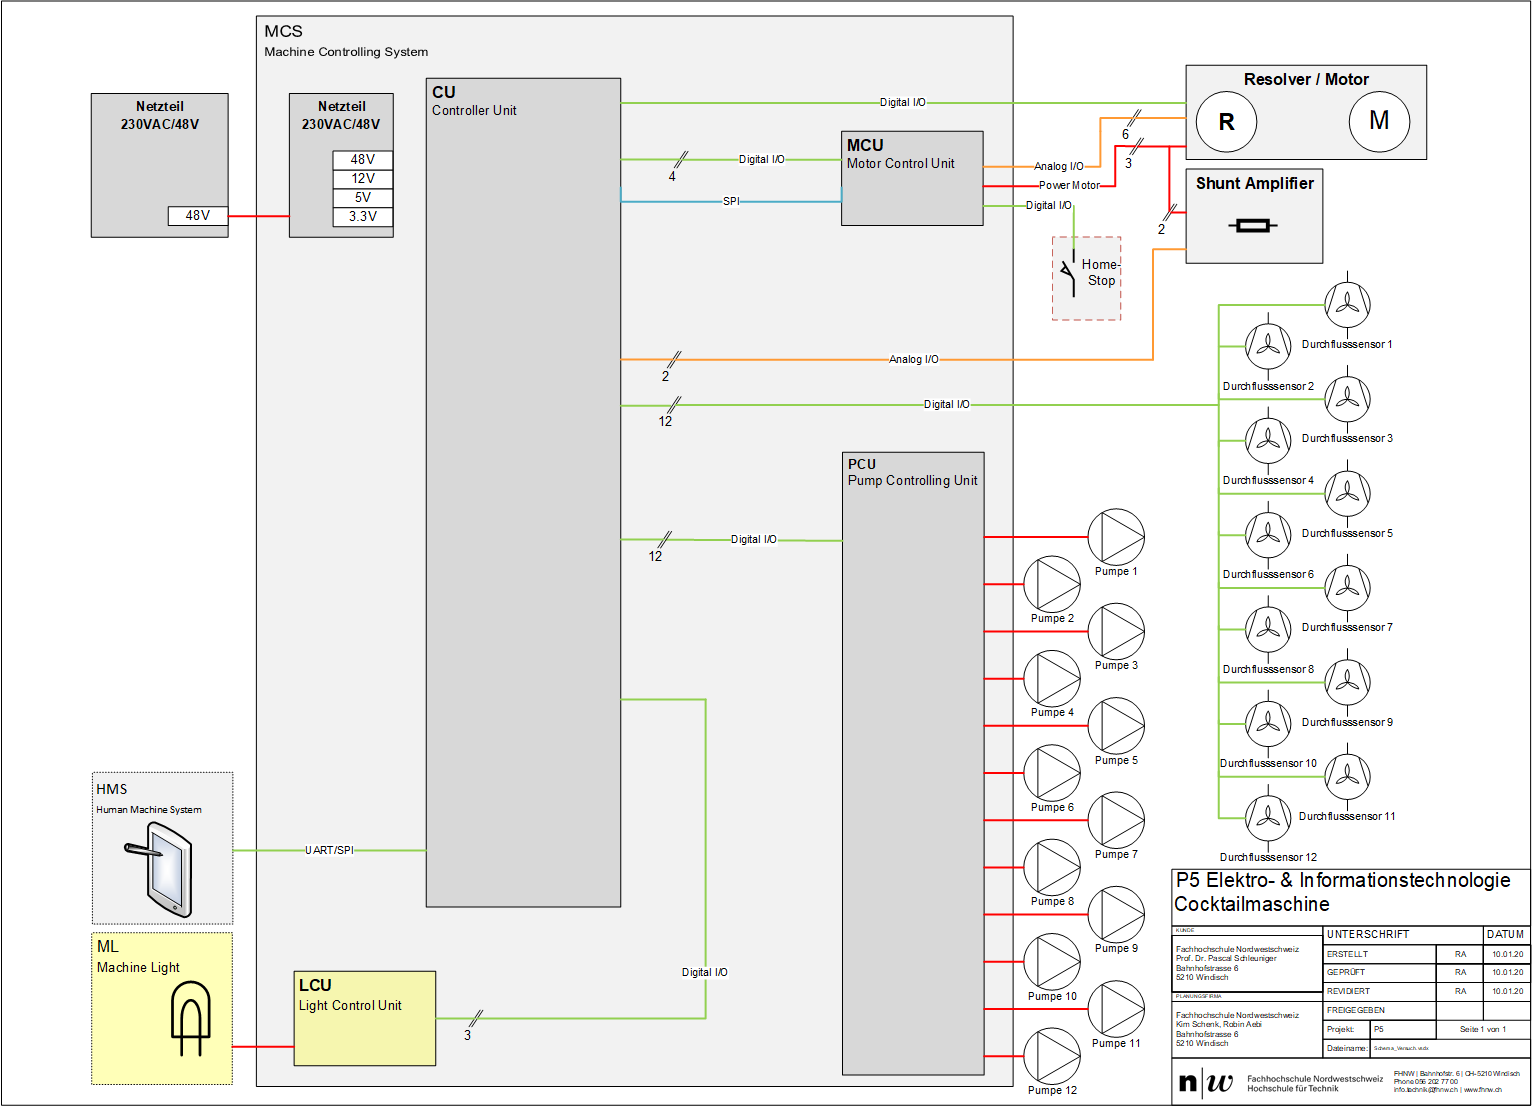
\includegraphics[height=100mm]{images/P5-Blockschema.png}
        \graphicscaption{Blockschema des PartyMixer's}
    \end{minipage}
}

\fscontent{
    \section{Die Aufgabe}
	Damit der PartyMixer ein Erfolg wird, mussten einige Dinge im Voraus abgeklärt werden. Dazu wurde eine ausführliche Recherche vorgenommen, welche den grundsätzlichen Aufbau dieser Maschine festlegte. Aufgrund dieser Entscheidungsfindung konnten im Anschluss die dazugehörigen Komponenten bestimmt und evaluiert werden.
    \section{Aufbau}
	Die Getränke sollen nicht an Ort und Stelle befüllt werden, was den Showeffekt erhöht. Ziel ist, dass ein Glas via Förderband zu den einzelnen Getränken gefahren wird, wo es dann befüllt wird. Die Getränkeflaschen sollen dabei nicht sichtbar verstaut sein. Eine einfach gestaltete Bedienung ist für den Benutzer wünschenswert. Aus diesem Grund soll der PartyMixer via Touchscreen Display bedient werden können.                   
    \section{Komponenten}   
    Das Herz des PartyMixer's bildet ein Mikrocontroller. Dieser soll die einzelnen Peripherien sauber ansteuern und auslesen. Dazu gehören ein Motor, welcher ein Förderband bewegt, die Pumpen, welche die Getränke befördern, die Durchflussmesgräte, welche den Durchfluss bestimmen sowie ein Touchscreen Display, welches als Benutzerschnittstelle fungiert.    
}

\infobox{Features}{%
    \footnotesize
    \setlength\tabcolsep{2pt}
    \begin{tabular}{lp{100mm}lp{0mm}}
    \bfseries Komponenten  		&                         			& 	  &\\
   \\
    Speisungen:	&  \SI{48}{\volt} / \SI{12}{\volt} / \SI{5}{\volt} / \SI{3.3}{\volt}			  																												&     &\\
    
    Mikrokontroller:      	& ATmega2560-16AU					&     &\\
    Pumpen:			  		& Vakuum-Membranpumpen   \SI{12}{\volt}     			&     &\\
  	Durchflussmessgeräte:	& Mechanisch-Volumetrisch \SI{5}{\volt}    	&     &\\ 		        		
    Motor:         			& AKM 22h \SI{48}{\volt}            &     &\\
    Display:                & Nextion NX8048T070 \SI{5}{\volt} 	&     &\\
    \end{tabular}
}
